%\documentclass[9pt]{scrartcl}
\documentclass[a4paper]{article}
\usepackage[]{amsmath}
\usepackage{tikz}
\usetikzlibrary{positioning}
%\usepackage{helvet}
\usepackage{listings}
\usepackage{geometry}
%\geometry{textheight=\paperheight, noheadfoot, nomarginpar}
\usetikzlibrary{positioning,shapes,shadows}
\renewcommand{\familydefault}{\sfdefault}

\tikzstyle{abstract}=[rectangle, draw=black, fill=gray!20, text centered,  text=black, text width=12.5mm]
\tikzstyle{spacestyle}=[rectangle, draw=black, fill=gray!20, text centered,  text=black, text width=50mm]

\lstset{
        language=python,
        basicstyle=\fontencoding{T1}\ttfamily,
        commentstyle=\color{gray},
        keywordstyle=\color{OliveGreen},
        frame=single,
        backgroundcolor=\color{lightlightgray},
        tabsize=2,
        %deletestring=[d]",
        %escapechar=\%,
        numbers=left,
        showstringspaces=false,
}
\usepackage[explicit]{titlesec} 
\titleformat{\section}{\normalfont\Large\bfseries}{}{0em}{#1}
\titleformat{\subsection}{\normalfont\bfseries}{}{0em}{--#1}

\newcommand{\mykey}[2]{%
\begin{tikzpicture} \node (Item) [abstract, minimum size=12.5mm, align=center]
{\vrule height 12pt depth 8pt width 0pt\textbf{#1} \\\vrule height 6pt depth 8pt width 0pt\parbox{1.25cm}{\centering{\fontsize{6pt}{8pt}\selectfont{#2}}}};%
\end{tikzpicture}}


\begin{document}
\begin{center}
\Large{Diagram}
\end{center}
\noindent%


\section {System diagram}
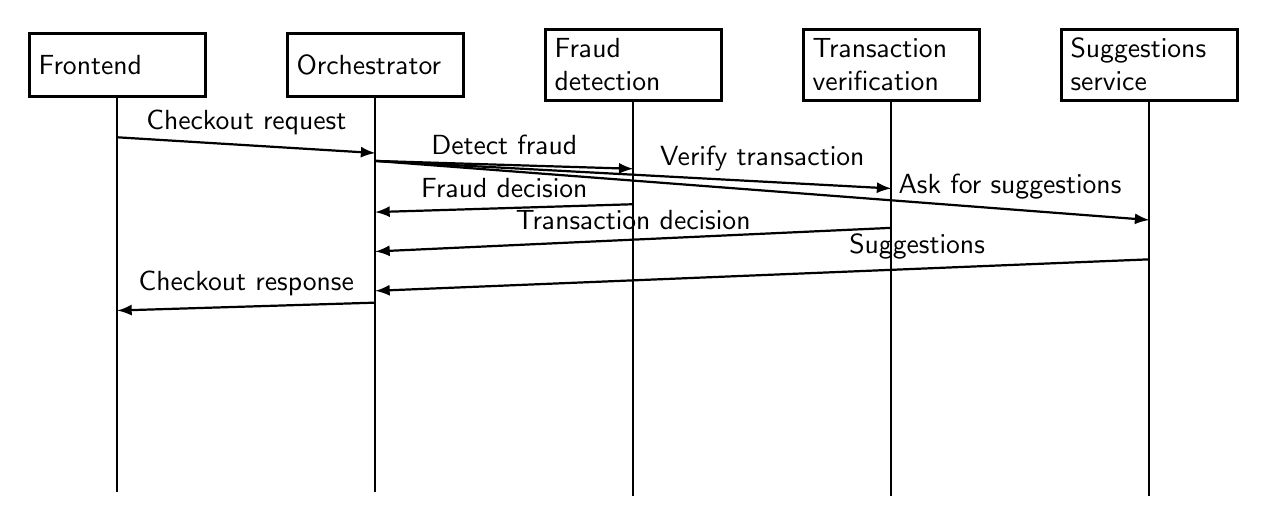
\begin{tikzpicture}

% Frontend
\node [draw,
	minimum width=2cm,
	minimum height=0.8cm,
	text width=2cm,
	very thick,
]  (frontend) {
Frontend
};

% Orchestrator
\node [draw,
	minimum width=2cm,
	minimum height=0.8cm,
	text width=2cm,
	very thick,
	right = 1cm of frontend
]  (orchestrator) {
Orchestrator
};
%\node [draw,
%	minimum width=2cm,
%	text width=5cm,
%	below = 0cm of widefield
%]  (framesWF) {
%8085: WF frames publisher
%};
%\node [draw,
%	minimum width=2cm,
%	text width=5cm,
%	below = 0cm of framesWF
%]  (detWF) {
%8089: WF detections publisher
%};
%\node [draw,
%	minimum width=2cm,
%	text width=5cm,
%	below = 0cm of detWF
%]  (confWF) {
%8086: WF conf subscriber
%};
%\node [draw,
%	minimum width=2cm,
%	text width=5cm,
%	below = 0cm of confWF
]%  (cropsWF) {
%8090: WF crops publisher
%};

% Fraud detection
\node [draw,
	minimum width=2cm,
	minimum height=0.8cm,
	text width=2cm,
	very thick,
	right = 1cm of orchestrator
]  (fraud_detection) {
Fraud\\detection
};
%\node [draw,
%	minimum width=2cm,
%	text width=5cm,
%	below = 0cm of shark
%]  (control) {
%8087: Controls subscriber
%};
%\node [draw,
%	minimum width=2cm,
%	text width=5cm,
%	below = 0cm of control
%]  (feedback) {
%8088: Control feedback publisher
%};

% Transaction verifier
\node [draw,
	minimum width=2cm,
	minimum height=0.8cm,
	text width=2cm,
	very thick,
	right = 1cm of fraud_detection
]  (transaction_verification) {
Transaction verification
};
%\node [draw,
%	minimum width=2cm,
%	text width=5cm,
%	below = 0cm of midfield
%]  (framesMF) {
%8105: MF frames publisher
%};
%\node [draw,
%	minimum width=2cm,
%	text width=5cm,
%	below = 0cm of framesMF
%]  (detMF) {
%8109: MF detections publisher
%};
%\node [draw,
%	minimum width=2cm,
%	text width=5cm,
%	below = 0cm of detMF
%]  (confMF) {
%8106: MF conf subscriber
%};

% Suggestions service
\node [draw,
	minimum width=2cm,
	minimum height=0.8cm,
	text width=2cm,
	very thick,
	right = 1 cm of transaction_verification
] (suggestions_service) {
Suggestions service
};

% Arrows with text label

%\draw[-latex, thick] (framesWF.west) -| (controls.south);
%\draw[-latex, thick] ([yshift=1mm]detWF.west) -| ([xshift=.3cm]controls.south);
%\draw[-latex, thick] ([yshift=-1mm]detWF.west) -| (shark.north);
%\draw[-latex, thick] ([xshift=.6cm]controls.south) |- (confWF.west);
%\draw[-latex, thick] (cropsWF.west) -| ([xshift=.9cm]controls.south);

%\draw[-latex, thick] (control.east) -| (4,0) |- ([yshift=1mm]controls.east);
%\draw[-latex, thick] ([yshift=-1mm]controls.east) -| (5,-1) |- (feedback.east);

%\draw[-latex, thick] (framesMF.west) -| (6,-3) -| ([xshift=-3mm]controls.south);
%\draw[-latex, thick] ([yshift=1mm]detMF.west) -| (5.5,-3.5) -| ([xshift=-8mm]controls.south);
%\draw[-latex, thick] ([yshift=-1mm]detMF.west) -| (5.2,-6) |- (shark.east);
%\draw[-latex, thick] ([xshift=-13mm]controls.south) |- (4.5, -4) |- (confMF.west);

%\draw[thick] (frontend) -- (orchestrator) node[midway, right] {HTTP};
%\draw[thick] (orchestrator.east) -- (fraud_detection.west) node[midway, above] {RPC};
%\draw[thick] (orchestrator.east) -- (transaction_verification.west) node[midway, above] {RPC};
%\draw[thick] (orchestrator.east) -- (suggestions_service.west) node[midway, above] {RPC};

\draw[thick] (frontend.south) -- ([yshift=-5cm] frontend.south);
\draw[thick] (orchestrator.south) -- ([yshift=-5cm] orchestrator.south);
\draw[thick] (fraud_detection.south) -- ([yshift=-5cm] fraud_detection.south);
\draw[thick] (transaction_verification.south) -- ([yshift=-5cm] transaction_verification.south);
\draw[thick] (suggestions_service.south) -- ([yshift=-5cm] suggestions_service.south);

\draw[-latex, thick] ([yshift=-0.5cm] frontend.south) -- ([yshift=-0.7cm] orchestrator.south) node[midway,above] {Checkout request};

\draw[-latex, thick] ([yshift=-0.8cm] orchestrator.south) -- ([yshift=-0.85cm] fraud_detection.south) node[midway,above] {Detect fraud};
\draw[-latex, thick] ([yshift=-0.8cm] orchestrator.south) -- ([yshift=-1.1cm] transaction_verification.south) node[pos=0.75,above] {Verify transaction};
\draw[-latex, thick] ([yshift=-0.8cm] orchestrator.south) -- ([yshift=-1.5cm] suggestions_service.south) node[pos=0.82,above] {Ask for suggestions};

\draw[-latex, thick] ([yshift=-1.3cm] fraud_detection.south) -- ([yshift=-1.45cm] orchestrator.south) node[midway,above] {Fraud decision};
\draw[-latex, thick] ([yshift=-1.6cm] transaction_verification.south) -- ([yshift=-1.95cm] orchestrator.south) node[midway,above] {Transaction decision};
\draw[-latex, thick] ([yshift=-2cm] suggestions_service.south) -- ([yshift=-2.45cm] orchestrator.south) node[pos=0.3,above] {Suggestions};

\draw[-latex, thick] ([yshift=-2.6cm] orchestrator.south) -- ([yshift=-2.7cm] frontend.south) node[midway,above] {Checkout response};

\end{tikzpicture}


\end{document}